\documentclass[10pt,conference]{IEEEtran}
\IEEEoverridecommandlockouts

\usepackage{iftex}
\ifXeTeX
  \usepackage{fontspec}
  \setmainfont{Times New Roman}
\else\ifLuaTeX
  \usepackage{fontspec}
  \setmainfont{Times New Roman}
\else
  \usepackage{newtxtext,newtxmath}
\fi\fi

\usepackage{cite}
\usepackage{amsmath}
\let\Bbbk\relax
\usepackage{amssymb,amsfonts}
\usepackage{algorithmic}
\usepackage{graphicx}
\usepackage{textcomp}
\usepackage{xcolor}
\usepackage{booktabs}
\usepackage[hidelinks]{hyperref}

\hyphenation{op-tical net-works semi-conduc-tor}

\setlength{\parskip}{0pt}
\setlength{\abovedisplayskip}{5pt plus 1pt minus 1pt}
\setlength{\belowdisplayskip}{5pt plus 1pt minus 1pt}
\setlength{\abovedisplayshortskip}{2pt plus 1pt minus 1pt}
\setlength{\belowdisplayshortskip}{2pt plus 1pt minus 1pt}
\setlength{\floatsep}{6pt plus 2pt minus 1pt}
\setlength{\textfloatsep}{8pt plus 2pt minus 2pt}
\setlength{\intextsep}{6pt plus 2pt minus 1pt}
\setlength{\abovecaptionskip}{4pt plus 1pt minus 1pt}
\setlength{\belowcaptionskip}{3pt plus 1pt minus 1pt}

\makeatletter
\renewcommand\section{\@startsection{section}{1}{\z@}%
  {1.4ex \@plus 0.4ex \@minus 0.2ex}%
  {0.7ex \@plus 0.2ex}%
  {\normalfont\fontsize{12pt}{14.4pt}\selectfont\bfseries\centering}}
\renewcommand\subsection{\@startsection{subsection}{2}{\z@}%
  {1.1ex \@plus 0.3ex \@minus 0.2ex}%
  {0.5ex \@plus 0.1ex}%
  {\normalfont\fontsize{12pt}{14.4pt}\selectfont\bfseries}}
\renewcommand\subsubsection{\@startsection{subsubsection}{3}{\z@}%
  {0.9ex \@plus 0.2ex \@minus 0.1ex}%
  {0.4ex \@plus 0.1ex}%
  {\normalfont\fontsize{12pt}{14.4pt}\selectfont\bfseries}}

\long\def\@makecaption#1#2{%
  \vskip\abovecaptionskip
  \sbox\@tempboxa{\fontsize{9pt}{11pt}\selectfont #1: #2}%
  \ifdim \wd\@tempboxa >\hsize
    {\fontsize{9pt}{11pt}\selectfont #1: #2\par}
  \else
    \global \@minipagefalse
    \hb@xt@\hsize{\hfil\box\@tempboxa\hfil}%
  \fi
  \vskip\belowcaptionskip}
\makeatother

\begin{document}

\title{\fontsize{16pt}{19.2pt}\selectfont\bfseries Automated Syslog Anomaly Detection and Explainable Analysis for Server Security}

\author{
\IEEEauthorblockN{
\fontsize{12pt}{14.4pt}\selectfont\bfseries
Prof. Archana T Chawhan\textsuperscript{1},
Pallavi R\textsuperscript{2},
Pradeep Sunkad\textsuperscript{2},
Sahana O M\textsuperscript{2}, and
Pramod P Jain\textsuperscript{2}
}
\IEEEauthorblockA{
\fontsize{10pt}{12pt}\selectfont\normalfont
\textsuperscript{1,2}Department of Computer Science and Engineering\\
Bapuji Institute of Engineering and Technology\\
Davanagere--577004, Karnataka, India
}
}

\maketitle

\begin{abstract}
\normalfont\fontsize{10pt}{12pt}\selectfont
Server system logs (syslogs) record critical security telemetry, yet manual inspection and static keyword rules fail against evolving threats while generating severe alert fatigue. In this paper, we present \emph{Smart-Log}, an automated, unsupervised, and explainable log anomaly detection framework tailored for server security. Smart-Log parses raw syslog streams, cleans malformed entries, and extracts an 8-dimensional behavioral feature representation over temporal sliding windows ($W=5$). For anomaly detection, an unsupervised Isolation Forest model functions as the primary detector, while a secondary One-Class Support Vector Machine (SVM) provides geometric cross-validation, establishing a four-state consensus triage hierarchy. Model interpretability is provided via TreeSHAP feature attributions alongside a standard-score fallback heuristic for incident investigation. Ground-truth labels are not used as model inputs, optimization targets, or preprocessing statistics; they are used only for stratified partitioning and final evaluation. Evaluated under strictly train-isolated preprocessing, Isolation Forest achieves 92.33\% accuracy, 84.35\% F1-score, and 0.9863 ROC-AUC on a constructed 1,000-sample scenario test split (300 samples), and 97.30\% accuracy, 0.9687 ROC-AUC, a low 1.24\% false positive rate, and an 81.67\% consensus agreement rate on a 10,000-sample HDFS benchmark test split (3,000 samples).
\end{abstract}

\begin{IEEEkeywords}
\normalfont\fontsize{10pt}{12pt}\selectfont
Anomaly detection, behavioral feature engineering, explainable artificial intelligence (XAI), Isolation Forest, One-Class SVM, server security, SHAP, system logs (syslog).
\end{IEEEkeywords}

\section{Introduction}
\label{sec:introduction}
Server system logs (syslogs) constitute the primary operational and security telemetry generated by operating system kernels, background daemons, network services, and application workloads \cite{b1}. In enterprise server clusters and cloud infrastructures, logs continuously record operational states, authorization attempts, resource allocation milestones, and hardware exceptions. Analyzing these log streams is critical for detecting unauthorized privilege escalation, distributed brute-force attacks, resource exhaustion, and critical service crashes before they compromise system availability or data integrity \cite{b2}.

Despite their diagnostic value, extracting actionable security intelligence from raw log streams presents significant challenges. Modern production environments generate large volumes of unstructured or semi-structured log messages daily. Traditional log management infrastructures rely heavily on Security Information and Event Management (SIEM) systems configured with static regex patterns and keyword search rules (e.g., matching keywords such as \texttt{"error"}, \texttt{"failed"}, or \texttt{"fatal"}) \cite{b3}. Such rule-based approaches exhibit fundamental limitations:
\begin{enumerate}
\item \textbf{Inability to Generalize:} Static keyword filters cannot detect novel or zero-day anomalies that do not match predefined signature patterns.
\item \textbf{Alert Fatigue:} Benign background warnings (e.g., transient network retries or scheduled maintenance tasks) frequently trigger false positives, overwhelming security analysts with low-fidelity alerts.
\item \textbf{Lack of Contextual and Temporal Awareness:} Individual log lines evaluated in isolation fail to capture behavioral trends, such as connection bursts or progressive authentication failures spanning multiple consecutive seconds.
\end{enumerate}

To overcome these constraints, machine learning techniques have been increasingly applied to log anomaly detection \cite{b6, b16}. However, supervised learning algorithms require large volumes of precisely labeled normal and anomalous log sequences, which are rarely available in live production settings due to the high cost of manual annotation and the evolving nature of cyber threats. Consequently, unsupervised anomaly detection models, which learn the intrinsic distribution of baseline system operations without requiring ground-truth labels, are necessary for practical deployment.

Furthermore, deploying machine learning models in security environments requires transparency. Black-box anomaly scores that flag an event without providing explanatory rationale leave incident responders unable to rapidly verify the threat or formulate mitigation strategies \cite{b6, b8}. Therefore, incorporating post-hoc explainability methods that attribute anomaly scores to specific behavioral features is essential for practical security operations.

In this paper, we present \textbf{Smart-Log}, an automated, unsupervised, and explainable log anomaly detection framework tailored for server security. The proposed framework transforms raw, unstructured log messages into an 8-dimensional behavioral feature space over sliding temporal windows, executes primary anomaly detection via Isolation Forest, provides secondary cross-validation with One-Class SVM, and explains individual anomaly flags using feature attribution techniques.

The key contributions of this paper are summarized as follows:
\begin{itemize}
\item We design a log preprocessing and behavioral feature engineering pipeline that parses raw system logs into standardized fields, cleans invalid entries, and extracts an exact 8-dimensional behavioral feature representation capturing event frequency, sequence length, error patterns, authentication attempts, and warning counts.
\item We implement an unsupervised detection architecture combining an Isolation Forest primary detector with a secondary One-Class SVM validator to provide a four-state consensus triage hierarchy that separates routine anomaly detections from high-confidence consensus escalations.
\item We integrate a feature attribution engine using TreeSHAP where available, supported by a fallback standard-score deviation attribution heuristic, to explain model predictions, assign operational severity bands, and generate feature-level diagnostic information to support alert triage.
\item We conduct empirical evaluations across two distinct experimental environments: a constructed 1,000-sample syslog scenario evaluation dataset and a 10,000-sample slice of the real-world HDFS LogHub benchmark dataset, validating performance, ROC-AUC, PR-AUC, and precision-recall trade-offs under strictly train-isolated preprocessing.
\end{itemize}

The remainder of this paper is structured as follows. Section~\ref{sec:related_work} reviews related work in log analysis and explainable security. Section~\ref{sec:proposed_system} details the Smart-Log system architecture and preprocessing pipeline. Section~\ref{sec:anomaly_detection} presents the primary detection and secondary consensus triage mechanisms. Section~\ref{sec:explainability} describes the feature attribution and explainability module. Section~\ref{sec:dataset_setup} outlines the datasets and experimental setup. Section~\ref{sec:results} presents the empirical results and discussion. Section~\ref{sec:limitations} discusses system limitations, and Section~\ref{sec:conclusion} concludes the paper.

\section{Related Work}
\label{sec:related_work}

\subsection{Rule-Based and Signature-Based Log Analysis}
Early approaches to server log management relied primarily on expert-crafted regular expressions, static thresholding, and string pattern matching \cite{b7}. Traditional rule-based and signature-based log analysis frameworks parse incoming event streams against predefined rule tables and static pattern libraries to identify known error strings or unauthorized access attempts \cite{b7}. To structure raw textual logs, automated log parsing can transform free-form log messages into structured event representations \cite{b13, b15}. While these parsers convert free-form text into structured event identifiers, signature-based detection systems remain inherently rigid: they cannot detect novel failure modes, fail to capture multi-event temporal correlations, and require continual manual rule maintenance by domain experts.

\subsection{Machine Learning-Based Log Anomaly Detection}
To improve adaptability, researchers transitioned to machine learning methodologies. Earlier machine-learning and representation-learning studies applied neural network classifiers and deep autoencoders to network intrusion records and cybersecurity logs to separate normal traffic from anomalous activity \cite{b20, b21}. With the advent of deep learning, sequence-based neural architectures, including DeepLog \cite{b17}, LogAnomaly \cite{b18}, and LogBERT \cite{b19}, modeled sequential event dependencies to predict the likelihood of subsequent log keys. Advanced representations employing prototypical networks \cite{b4}, large language models \cite{b5}, graph-based representations \cite{b11}, and neural architectures based on LSTM, GRU, or CNN mechanisms \cite{b23, b24} further extended contextual modeling capabilities. Although neural architectures achieve strong sequential modeling, they incur high computational training costs, require substantial memory footprints, and typically necessitate supervised or semi-supervised fine-tuning.

Unsupervised ensemble methods, particularly Isolation Forest \cite{b14, b22}, and boundary-estimation techniques, such as One-Class Support Vector Machines (OCSVM), have emerged as efficient alternatives for anomaly detection in high-dimensional data. Isolation Forest explicitly isolates anomalies through recursive random partitioning rather than constructing profiles of normal instances, making it computationally efficient and robust against high-dimensional noise. One-Class SVM maps data points into a reproducing kernel Hilbert space to construct a maximum-margin hyperplane enclosing baseline vectors. Deploying these complementary algorithms provides both fast tree-based partitioning and kernel geometric validation.

\subsection{Explainable AI for Security}
The integration of Explainable Artificial Intelligence (XAI) in cybersecurity has gained substantial attention to address the black-box nature of machine learning models \cite{b6, b8, b12, b16}. Model-agnostic local explanation frameworks quantify feature importance for individual predictions. For tree-based ensemble models, TreeSHAP computes Shapley values by leveraging the internal decision-tree graph structure. Integrating feature attribution with structured diagnostic summaries provides a practical bridge between automated anomaly detection and operational incident response.

\section{Proposed System Architecture}
\label{sec:proposed_system}

\subsection{System Architecture Overview}
The overall architecture of the proposed \textbf{Smart-Log} framework is illustrated in Fig.~\ref{fig_arch}. The system operates as a pipeline comprising four major functional layers:
\begin{enumerate}
\item \textbf{Ingestion and Parsing Layer:} Ingests raw syslog streams and extracts structured metadata fields via regular expressions.
\item \textbf{Preprocessing and Feature Engineering Layer:} Performs missing-value imputation, numerical bounding, and projects log records into an 8-dimensional canonical behavioral space over sliding temporal windows.
\item \textbf{Detection and Validation Layer:} Evaluates feature vectors using an unsupervised Isolation Forest as the primary detector and cross-validates detections with One-Class SVM.
\item \textbf{Explainability and Alerting Layer:} Computes feature contribution attributions via TreeSHAP (with fallback support), assigns operational severity bands, and outputs diagnostic explanations alongside feature-level triage information.
\end{enumerate}

\begin{figure*}[t]
\centering
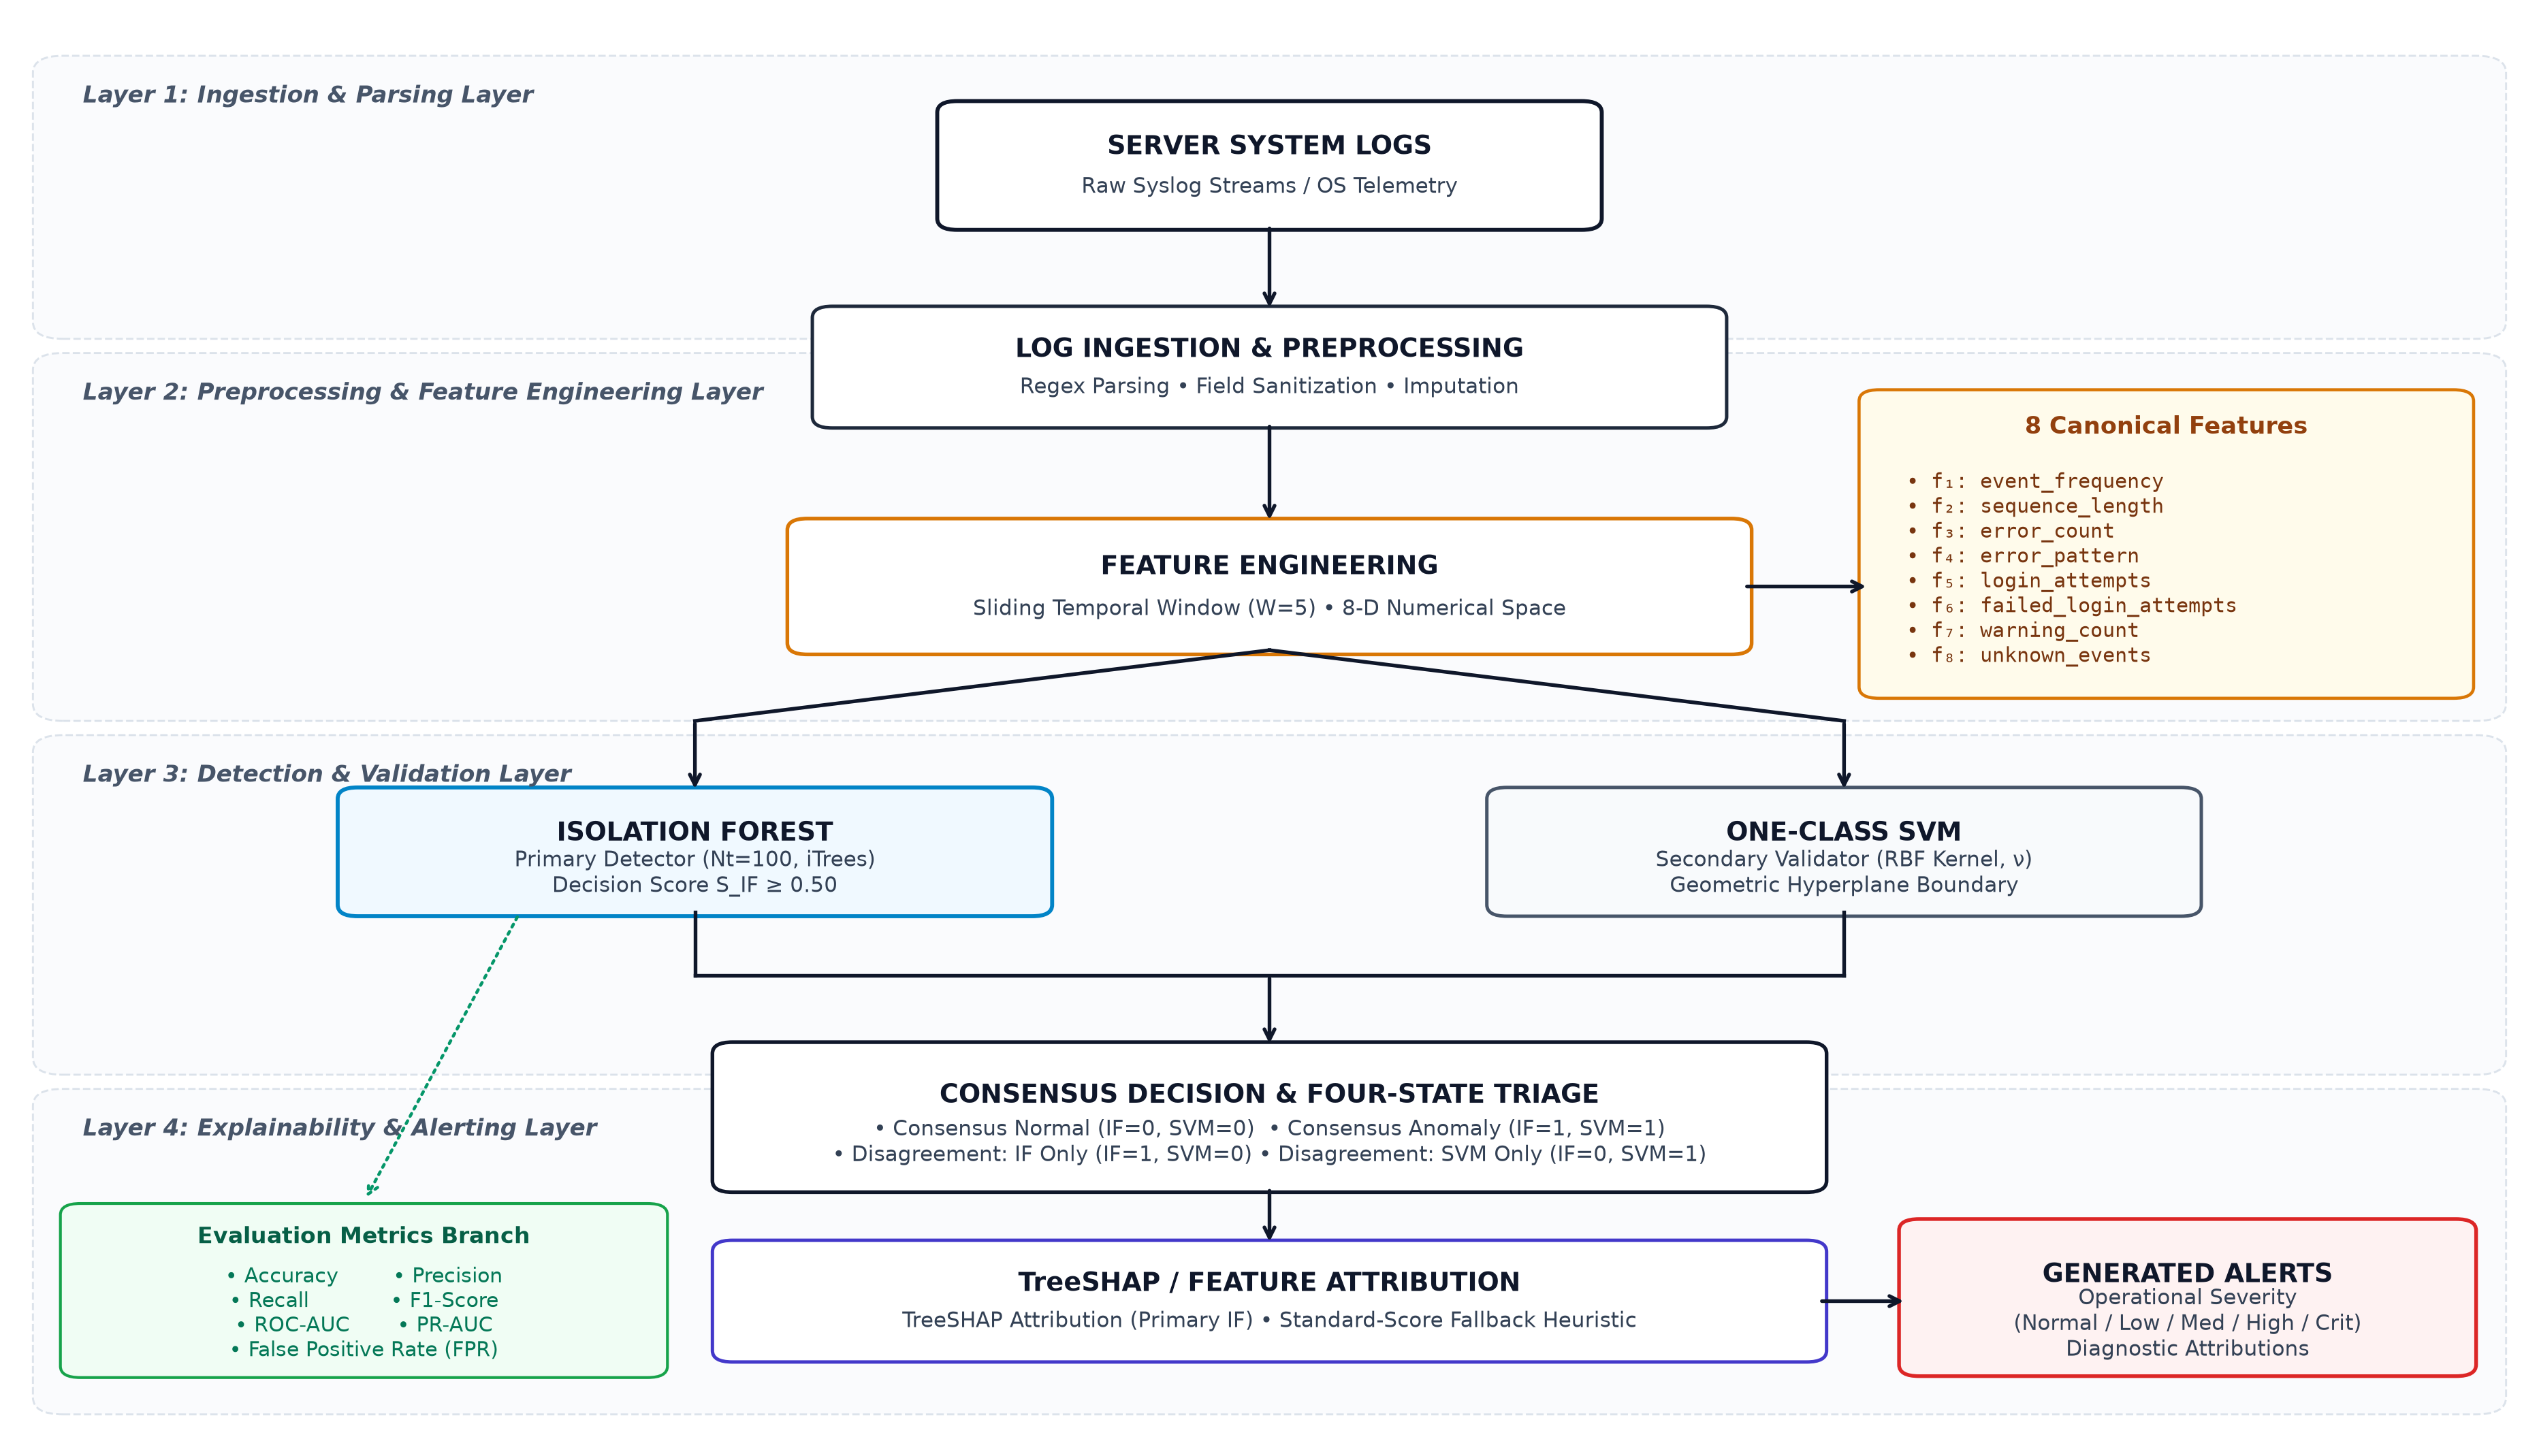
\includegraphics[width=0.92\textwidth]{fig_arch.png}
\caption{End-to-end system architecture of the proposed Smart-Log log anomaly detection and explainability framework, depicting log ingestion, preprocessing, behavioral feature extraction, dual-model detection, TreeSHAP attribution, alert triage, and offline evaluation.}
\label{fig_arch}
\end{figure*}

\subsection{Log Ingestion and Parsing}
Raw system logs arrive as unstructured text strings formatted according to standard syslog conventions or operating system event structures. The log parser utilizes regular expressions to extract attributes from each raw log entry:
\begin{equation}
\mathcal{L}_i = \langle t_i, h_i, s_i, \ell_i, m_i \rangle
\label{eq_log_tuple}
\end{equation}
where $t_i$ is the timestamp, $h_i$ represents the originating hostname or IP address (defaulting to \texttt{"localhost"} if absent), $s_i$ denotes the service or process identifier (defaulting to \texttt{"system"}), $\ell_i$ is the standardized log severity level, and $m_i$ represents the raw message payload.

The parser categorizes each log entry into standardized operational severity levels:
\begin{equation}
\ell_i \in \{\text{INFO}, \text{WARNING}, \text{ERROR}, \text{CRITICAL}\}
\end{equation}
Classification is performed by scanning message text and headers for status indicators (e.g., tokenizing strings containing \texttt{"ERROR"}, \texttt{"FAILED"}, \texttt{"EXCEPTION"}, or \texttt{"WARN"}).

\subsection{Data Cleaning and Normalization}
System log streams frequently contain malformed headers, missing fields, or invalid numerical records resulting from buffer truncation or network packet corruption. The data cleaning module enforces the following pipeline:
\begin{itemize}
\item \textbf{Field Sanitization:} Strips invalid whitespace, replaces missing hostnames with loopback defaults (\texttt{"localhost"}), and assigns generic fallback labels (\texttt{"system"}) to unparseable service channels.
\item \textbf{Missing and Invalid Value Imputation:} Evaluates extracted numerical attributes for missing values ($\text{NaN}$) and positive/negative infinity ($\pm\infty$). Data-dependent parameters, including median imputation values and finite-value clipping bounds, are fitted exclusively on the training partition and applied unchanged to the held-out test partition to guarantee train-isolated preprocessing.
\item \textbf{Extreme Value Bounding:} Applies finite-value clipping to prevent arithmetic overflow in downstream matrix calculations:
\begin{equation}
\hat{x}_{i,j} = \min\left(\max(x_{i,j}, \text{LB}_j), \text{UB}_j\right)
\end{equation}
where $\text{LB}_j$ and $\text{UB}_j$ denote the lower and upper operational bounds for feature $j$.
\end{itemize}

\subsection{Behavioral Feature Engineering}
To capture operational dynamics rather than isolated keywords, Smart-Log projects the sanitized log stream into an exact 8-dimensional numerical behavioral space $\mathbf{x}_i \in \mathbb{R}^8$ calculated over a sliding temporal window of size $W = 5$ surrounding the target event ($i-2$ to $i+2$). The eight canonical features are defined in Table~\ref{tab_features}.

\begin{table}[t]
\caption{The 8 Canonical Behavioral Features in Smart-Log}
\label{tab_features}
\centering
\resizebox{\columnwidth}{!}{%
\begin{tabular}{|c|l|p{5.5cm}|}
\hline
\textbf{\#} & \textbf{Feature Key} & \textbf{Description \& Context} \\
\hline
$f_1$ & \texttt{event\_frequency} & Number of log events within sliding temporal window ($W=5$). \\
$f_2$ & \texttt{sequence\_length} & Character length of log payload for raw syslogs; total event occurrences ($\sum_{i=1}^{29} E_i$) in HDFS evaluation adapter. \\
$f_3$ & \texttt{error\_count} & Count of error/critical events in sliding window for syslogs; fault template count plus baseline offset ($3.0 + \sum E_{\text{fault}}$) in HDFS adapter. \\
$f_4$ & \texttt{error\_pattern} & Categorical fault pattern for syslogs (0: Normal, 1: \texttt{FAILED}, 2: \texttt{NO FILE}, 3: \texttt{OOM}, 4: \texttt{DENIED}); binary fault indicator in HDFS adapter (1.0: fault absence / nominal, 0.0: fault presence). \\
$f_5$ & \texttt{login\_attempts} & Count of authentication/session initiation calls in syslogs ($0.0$ unpopulated channel for HDFS). \\
$f_6$ & \texttt{failed\_login\_attempts} & Count of rejected authentications in syslogs ($0.0$ unpopulated channel for HDFS). \\
$f_7$ & \texttt{warning\_count} & Number of warning-level log events in syslogs ($0.0$ unpopulated channel for HDFS). \\
$f_8$ & \texttt{unknown\_events} & Frequency of unmapped or unrecognized log events in syslogs ($0.0$ unpopulated channel for HDFS). \\
\hline
\end{tabular}%
}
\end{table}

The resulting feature matrix $\mathbf{X} \in \mathbb{R}^{N \times 8}$ is strictly verified to contain zero $\text{NaN}$ and zero infinite entries prior to ingestion by the machine learning models.

\section{Anomaly Detection and Consensus Triage}
\label{sec:anomaly_detection}

\subsection{Primary Detector: Isolation Forest}
Isolation Forest serves as the primary unsupervised anomaly detection engine governing operational decisions. Unlike profile-building algorithms that model normal points, Isolation Forest explicitly isolates anomalies through recursive random partitioning rather than constructing profiles of normal instances, making it computationally efficient and robust against high-dimensional noise.

During training, an ensemble of $N_t = 100$ isolation trees ($iTrees$) is constructed using recursive spatial partitioning with $max\_samples = \text{'auto'}$, $random\_state = 42$, and $n\_jobs = -1$. For evaluation, the contamination parameter was configured to match the known anomaly proportions of the respective evaluation datasets ($0.25$ for the constructed scenario evaluation; $0.0293$ for the HDFS benchmark). For each tree, a sub-sample $\mathcal{X}' \subset \mathbf{X}_{\text{train}}$ of size $\min(256, |\mathbf{X}_{\text{train}}|)$ is selected. At each node, a feature $q \in \{f_1, \dots, f_8\}$ is chosen uniformly at random, and a split point $p$ is selected uniformly at random within the range $[\min(\mathbf{X}_q), \max(\mathbf{X}_q)]$. The sample space is divided into left and right sub-nodes until either: (i) the tree reaches its maximum depth limit, (ii) $|X| \le 1$, or (iii) all data points have identical values.

The theoretical anomaly score $s(\mathbf{x}, n)$ for an 8-dimensional feature vector $\mathbf{x}$ across $n$ samples is derived from the average path length $\mathbb{E}(h(\mathbf{x}))$:
\begin{equation}
s(\mathbf{x}, n) = 2^{-\frac{\mathbb{E}(h(\mathbf{x}))}{c(n)}}
\label{eq_if_score}
\end{equation}
where $h(\mathbf{x})$ is the number of edges traversed from the root node to a leaf node, and $c(n)$ is the average path length of an unsuccessful search in a Binary Search Tree (BST):
\begin{equation}
c(n) = 2\left(\ln(n - 1) + \gamma\right) - \frac{2(n - 1)}{n}
\end{equation}
with $\gamma \approx 0.5772156649$ (Euler-Mascheroni constant).

In the operational implementation, the scikit-learn decision function is mapped into a normalized continuous score $\hat{S}_{\text{IF}}(\mathbf{x}) \in [0.0, 1.0]$:
\begin{equation}
\hat{S}_{\text{IF}}(\mathbf{x}) = \text{clip}\left(1.0 - \left(\text{decision\_function}(\mathbf{x}) + 0.5\right), 0.0, 1.0\right)
\label{eq_norm_score}
\end{equation}
A binary prediction flag is assigned using the operational threshold $\hat{S}_{\text{IF}}(\mathbf{x}) \ge 0.50$ (corresponding exactly to raw tree decision boundary $\text{decision\_function}(\mathbf{x}) \le 0.0$ and $\hat{y} = -1$).

\subsection{Secondary Validator: One-Class SVM}
To validate the primary detections and provide geometric boundary cross-checking, a One-Class Support Vector Machine (OCSVM) is deployed alongside the primary detector. One-Class SVM maps input vectors into a higher-dimensional feature space $\Phi(\mathbf{x})$ via a non-linear kernel function and constructs an optimal maximum-margin separating hyperplane that bounds the dense cluster of normal vectors away from the coordinate origin.

We configure the OCSVM using a Radial Basis Function (RBF) kernel with $\gamma = \text{'scale'}$ ($\gamma = \frac{1}{8\,\operatorname{Var}(\mathbf{X})}$) and $\nu$ parameter aligned with the dataset anomaly proportions ($\nu = 0.25$ for scenario evaluations; $\nu = 0.03$ for benchmark cluster traces):
\begin{equation}
K(\mathbf{x}, \mathbf{x}') = \exp\left(-\gamma \|\mathbf{x} - \mathbf{x}'\|^2\right)
\end{equation}
The optimization problem is formulated as:
\begin{equation}
\min_{\mathbf{w}, \boldsymbol{\xi}, \rho} \frac{1}{2}\|\mathbf{w}\|^2 + \frac{1}{\nu N}\sum_{i=1}^N \xi_i - \rho
\end{equation}
\begin{equation}
\text{subject to } \langle \mathbf{w}, \Phi(\mathbf{x}_i) \rangle \ge \rho - \xi_i, \quad \xi_i \ge 0, \quad \forall i=1,\dots,N
\end{equation}
where $\nu \in (0, 1]$ represents an upper bound on the fraction of training outliers and a lower bound on the number of support vectors.

\subsection{Consensus Decision Logic and Four-State Triage}
In the Smart-Log framework, the primary Isolation Forest detector governs operational anomaly detection decisions, while One-Class SVM acts as a secondary validator to establish a four-state consensus triage categorization:
\begin{enumerate}
\item \textbf{Consensus Normal ($\hat{y}_{\text{IF}} = 0, \hat{y}_{\text{SVM}} = 0$):} Both models agree that the log sequence reflects standard baseline operations.
\item \textbf{Consensus Anomaly ($\hat{y}_{\text{IF}} = 1, \hat{y}_{\text{SVM}} = 1$):} Security anomaly confirmed by both tree isolation and kernel envelope boundaries. Suitable for high-priority automated escalation.
\item \textbf{Disagreement -- IF Only ($\hat{y}_{\text{IF}} = 1, \hat{y}_{\text{SVM}} = 0$):} Event exhibits sparse tree isolation characteristics but remains within the broader SVM geometric manifold. Logged for standard operational review.
\item \textbf{Disagreement -- SVM Only ($\hat{y}_{\text{IF}} = 0, \hat{y}_{\text{SVM}} = 1$):} Event falls outside the kernel boundary but possesses normal tree path length. Logged for diagnostic audit.
\end{enumerate}

\section{Explainability and Feature Attribution}
\label{sec:explainability}

\subsection{Feature Attribution Engine}
To provide model transparency, Smart-Log incorporates a local feature attribution engine. For tree-based models, TreeSHAP is employed where library dependencies are satisfied to decompose the local model prediction into additive feature attribution values (Shapley values $\phi_j$):
\begin{equation}
f(\mathbf{x}) = \phi_0 + \sum_{j=1}^{M} \phi_j(\mathbf{x})
\label{eq_shap}
\end{equation}
where $\phi_0$ denotes the expected model output under the explainer's reference/background distribution, and $\phi_j(\mathbf{x}) \in \mathbb{R}$ represents the contribution of feature $j$ toward pushing the anomaly score above or below the baseline.

Shapley-value-based feature attributions are computed using TreeSHAP for supported evaluation batches ($N \le 300$). When TreeSHAP is constrained by batch size ($N > 300$, where samples $0 \dots 299$ use TreeSHAP and remaining samples use fallback), runtime exceptions, or missing library dependencies, the system applies a normalized standard-score deviation heuristic to assign relative feature importance:
\begin{equation}
\phi_j^{\text{fallback}} = \left(\frac{z_j}{\sum_{k=1}^8 |z_k| + 10^{-5}}\right) \cdot \left(\hat{S}_{\text{IF}}(\mathbf{x}) - 0.5\right)
\end{equation}
where:
\begin{equation}
z_j = \frac{x_j - \mu_j}{\sigma_j + 10^{-5}}
\end{equation}
with $\mu_j$ and $\sigma_j$ representing the mean and standard deviation of feature $j$ across the training distribution. The fallback provides attribution coverage when exact TreeSHAP computation is unavailable; these values should be interpreted as heuristic relative feature contributions rather than Shapley values.

\subsection{Sample-Specific Interpretation and Severity Alerts}
The computed attributions are ranked by absolute magnitude to identify the top primary drivers of the anomaly:
\begin{equation}
\mathcal{R}_3(\mathbf{x}) = \operatorname{Top3}_{j \in \{1,\dots,8\}} |\phi_j(\mathbf{x})|
\end{equation}
where $\operatorname{Top3}$ extracts the indices of the three features with the largest absolute attribution magnitudes. Smart-Log maps the normalized score $\hat{S}_{\text{IF}}$ and top attributions into configurable operational severity bands, as summarized in Table~\ref{tab_severity}.

\begin{table}[t]
\caption{Operational Severity Bands and Triage Guidance}
\label{tab_severity}
\centering
\resizebox{\columnwidth}{!}{%
\begin{tabular}{|c|c|c|p{4.2cm}|}
\hline
\textbf{Score} & \textbf{Flag} & \textbf{Severity} & \textbf{Triage / Alert Guidance} \\
\hline
$[0.00, 0.49]$ & Normal ($0$) & \texttt{Normal} & Routine background logging. \\
$[0.50, 0.55]$ & Anomaly ($1$) & \texttt{Low} & Routine audit review. \\
$[0.56, 0.70]$ & Anomaly ($1$) & \texttt{Medium} & Service inspection guidance. \\
$[0.71, 0.85]$ & Anomaly ($1$) & \texttt{High} & Elevated security notification. \\
$[0.86, 1.00]$ & Anomaly ($1$) & \texttt{Critical} & Immediate alert escalation. \\
\hline
\end{tabular}%
}
\end{table}

For each flagged anomaly, the system formats a structured natural-language summary combining feature values, attribution rankings, and feature-level diagnostic information to support alert triage.

\section{Datasets and Experimental Setup}
\label{sec:dataset_setup}

To evaluate the system under controlled scenarios and real-world distributed cluster conditions, Smart-Log was evaluated across two distinct experimental environments:

\subsection{Constructed Syslog Scenario Evaluation Dataset}
This dataset contains $1,000$ structured syslog scenario records ($750$ normal baseline operations and $250$ anomalous security events) representing diverse server states, including SSH brute force, buffer overflow probes, out-of-memory kernel kills, and unauthorized privilege escalation. Labels are derived directly from deterministic scenario generation templates. The records are partitioned into a 70\% training split ($700$ samples) and a 30\% held-out test split ($300$ samples: $225$ normal, $75$ anomalous) using stratified sampling. Models were parameterized with $\text{contamination} = 0.25$ and $\nu = 0.25$ to match the scenario anomaly proportion.

\subsection{HDFS Distributed Cluster Benchmark Dataset}
To evaluate the framework on large-scale distributed telemetry, we utilize the standard Hadoop Distributed File System (HDFS) benchmark from the LogHub repository \cite{b9, b10}, which comprises $575,061$ block execution traces ($558,223$ normal and $16,838$ anomalous, representing a 2.93\% ground-truth anomaly ratio). For empirical evaluation, a stratified slice of $10,000$ block traces ($9,707$ normal, $293$ anomalous) is partitioned into a 70\% training split ($7,000$ samples) and a 30\% held-out test split ($3,000$ samples: $2,912$ normal, $88$ anomalous). Models were parameterized with $\text{contamination} = 0.0293$ and $\nu = 0.03$.

Because HDFS traces are provided as pre-parsed event-template counts rather than raw operating-system authentication logs, a dataset-specific adapter maps the native HDFS representation into the canonical Smart-Log feature schema. This mapping provides a common numerical interface for cross-dataset evaluation but does not imply identical semantic interpretation of every feature across datasets:
\begin{itemize}
\item \texttt{event\_frequency} is computed as the total event occurrences across all templates: $\sum_{i=1}^{29} E_i$.
\item \texttt{sequence\_length} is also assigned the total event count per block execution trace ($\sum_{i=1}^{29} E_i$), as HDFS input consists of pre-parsed count matrices rather than raw text character strings.
\item \texttt{error\_count} aggregates occurrences across designated fault templates ($E_4, E_7, E_{10}, E_{12}, E_{14}, E_{17}, E_{20}, E_{29}$) with an adapter baseline offset of $3.0$ derived from the normal median baseline:
\begin{equation}
\text{error\_count} = 3.0 + \sum_{k \in \{4,7,10,12,14,17,20,29\}} E_k
\end{equation}
\item \texttt{error\_pattern} is a binary fault-pattern encoding set to $1.0$ if designated fault templates sum to zero (fault absence / nominal) and $0.0$ otherwise (fault presence).
\item The four security-specific features (\texttt{login\_attempts}, \texttt{failed\_login\_attempts}, \texttt{warning\_count}, \texttt{unknown\_events}) are unpopulated channels set to zero ($0.0$) because HDFS block execution traces record distributed storage events rather than operating system user authentication telemetry.
\end{itemize}

\subsection{Evaluation Methodology and Metrics}
Ground-truth labels are not used as model inputs, optimization targets, or preprocessing statistics; they are used only for stratified partitioning and final evaluation. In both the constructed Syslog evaluation and the HDFS benchmark evaluation, the stratified 70/30 train-test split is performed prior to preprocessing; data-dependent preprocessing statistics (such as median imputation and finite upper bounds) are fitted exclusively on the training partition and applied unchanged to the held-out test partition to guarantee train-isolated preprocessing.

The evaluation metrics include Accuracy ($\text{Acc}$), Precision ($P$), Recall ($R$), F1-Score ($F_1$), Area Under the ROC Curve ($\text{ROC-AUC}$), Area Under the Precision-Recall Curve ($\text{PR-AUC}$), and False Positive Rate ($\text{FPR} = \frac{\text{FP}}{\text{FP} + \text{TN}}$).

\section{Results and Discussion}
\label{sec:results}

\subsection{Constructed Scenario Evaluation Results}
Table~\ref{tab_scenario_results} summarizes the performance metrics obtained on the held-out test split ($300$ samples) of the Constructed Syslog Scenario Evaluation Dataset.

\begin{table}[t]
\caption{Performance on Constructed Scenario Test Set (300 Samples)}
\label{tab_scenario_results}
\centering
\resizebox{\columnwidth}{!}{%
\begin{tabular}{|l|c|c|c|c|c|c|}
\hline
\textbf{Model / Setup} & \textbf{Prec.} & \textbf{Rec.} & \textbf{F1} & \textbf{ROC} & \textbf{PR} & \textbf{FPR} \\
\hline
Isolation Forest & 86.11\% & \textbf{82.67\%} & \textbf{84.35\%} & \textbf{0.9863} & \textbf{0.9511} & 4.44\% \\
One-Class SVM & 14.47\% & 14.67\% & 14.57\% & 0.4348 & 0.2411 & 28.89\% \\
Dual Consensus & \textbf{100.00\%} & 14.67\% & 25.58\% & 0.7404 & 0.4722 & \textbf{0.00\%} \\
\hline
\end{tabular}%
}
\end{table}

On this scenario benchmark, Isolation Forest demonstrates primary detection capability, identifying $62$ of $75$ true anomalies with only $10$ false positives ($\text{TN}=215, \text{FP}=10, \text{FN}=13, \text{TP}=62$), yielding an overall accuracy of 92.33\%, an F1-score of 84.35\%, an ROC-AUC of 0.9863, and a PR-AUC of 0.9511. In contrast, One-Class SVM produces $65$ false positives ($\text{FPR} = 28.89\%$, $\text{TN}=160, \text{FP}=65, \text{FN}=64, \text{TP}=11$). 

When evaluating the subset of events where both Isolation Forest and One-Class SVM agree on an anomaly (Dual Consensus state), the evaluation achieves 100.00\% Precision and 0.00\% False Positive Rate ($\text{TN}=225, \text{FP}=0, \text{FN}=64, \text{TP}=11$). However, this complete elimination of false alarms involves a significant trade-off in recall, which drops from 82.67\% to 14.67\%. Consequently, dual consensus is structured as an automated high-confidence escalation filter rather than a replacement for the primary anomaly detector.

\subsection{HDFS Benchmark Dataset Evaluation Results}
Table~\ref{tab_hdfs_results} presents the empirical evaluation results on the held-out test split ($3,000$ block traces) of the HDFS benchmark dataset.

\begin{table}[t]
\caption{Performance on HDFS Benchmark Test Set (3,000 Samples)}
\label{tab_hdfs_results}
\centering
\resizebox{\columnwidth}{!}{%
\begin{tabular}{|l|c|c|c|c|c|c|}
\hline
\textbf{Model / Setup} & \textbf{Prec.} & \textbf{Rec.} & \textbf{F1} & \textbf{ROC} & \textbf{PR} & \textbf{FPR} \\
\hline
Isolation Forest & \textbf{54.43\%} & \textbf{48.86\%} & \textbf{51.50\%} & \textbf{0.9687} & \textbf{0.4549} & \textbf{1.24\%} \\
One-Class SVM & 6.90\% & 47.73\% & 12.05\% & 0.5485 & 0.3033 & 19.47\% \\
\hline
\end{tabular}%
}
\end{table}

On the HDFS benchmark, the primary Isolation Forest detector achieves an overall accuracy of 97.30\%, an ROC-AUC of 0.9687, a PR-AUC of 0.4549, and a low false positive rate of 1.24\% ($\text{TN}=2876, \text{FP}=36, \text{FN}=45, \text{TP}=43$). The precision (54.43\%) and recall (48.86\%) reflect the highly imbalanced nature of real distributed log streams (2.93\% base anomaly rate). One-Class SVM flags 609 anomalies with 567 false positives ($\text{FPR} = 19.47\%$, $\text{TN}=2345, \text{FP}=567, \text{FN}=46, \text{TP}=42$).

The inter-model comparison across all $3,000$ HDFS test events demonstrates an overall agreement rate of \textbf{81.67\%} ($2,450$ agreeing predictions), with $2,381$ Consensus Normal events, $69$ Consensus Anomaly events, $10$ IF-only flags, and $540$ OCSVM-only flags.

\begin{figure}[t]
\centering
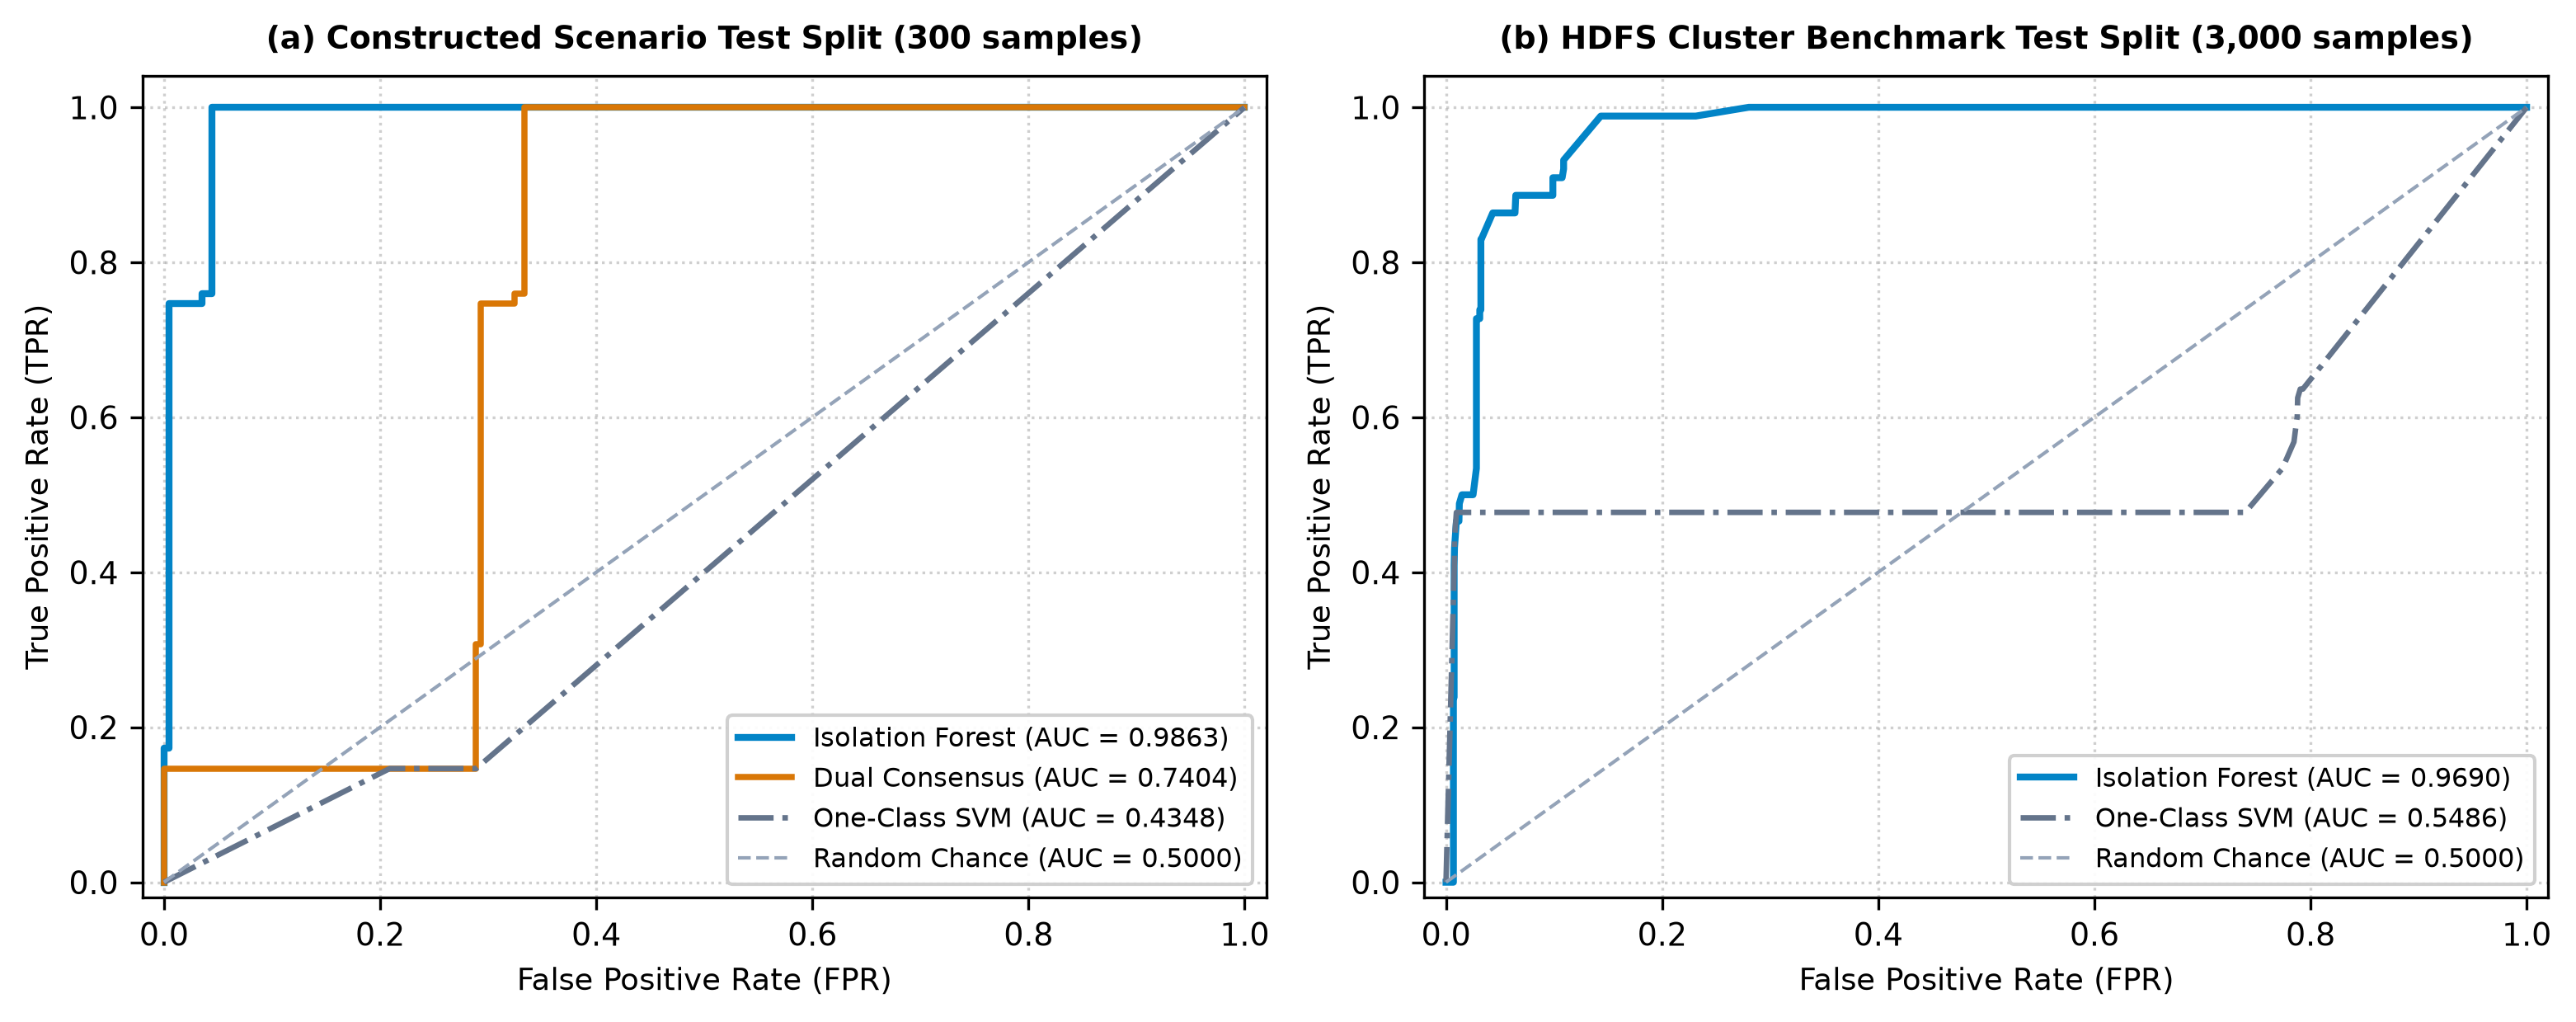
\includegraphics[width=\columnwidth]{fig_roc.png}
\caption{Receiver Operating Characteristic (ROC) curve comparison of the primary Isolation Forest detector, secondary One-Class SVM validator, and Dual Consensus triage across evaluation datasets.}
\label{fig_roc}
\end{figure}

\subsection{Feature Attribution and Interpretability Analysis}
Feature attribution analysis decomposes model anomaly scores into relative feature contributions ($\phi_i$). By inspecting the top three attributed features $\mathcal{R}_3(\mathbf{x})$, security operators can identify which behavioral dimensions drove the model anomaly score above the baseline threshold. This diagnostic attribution provides feature-level operational context for incident responders during alert triage.

\begin{figure}[t]
\centering
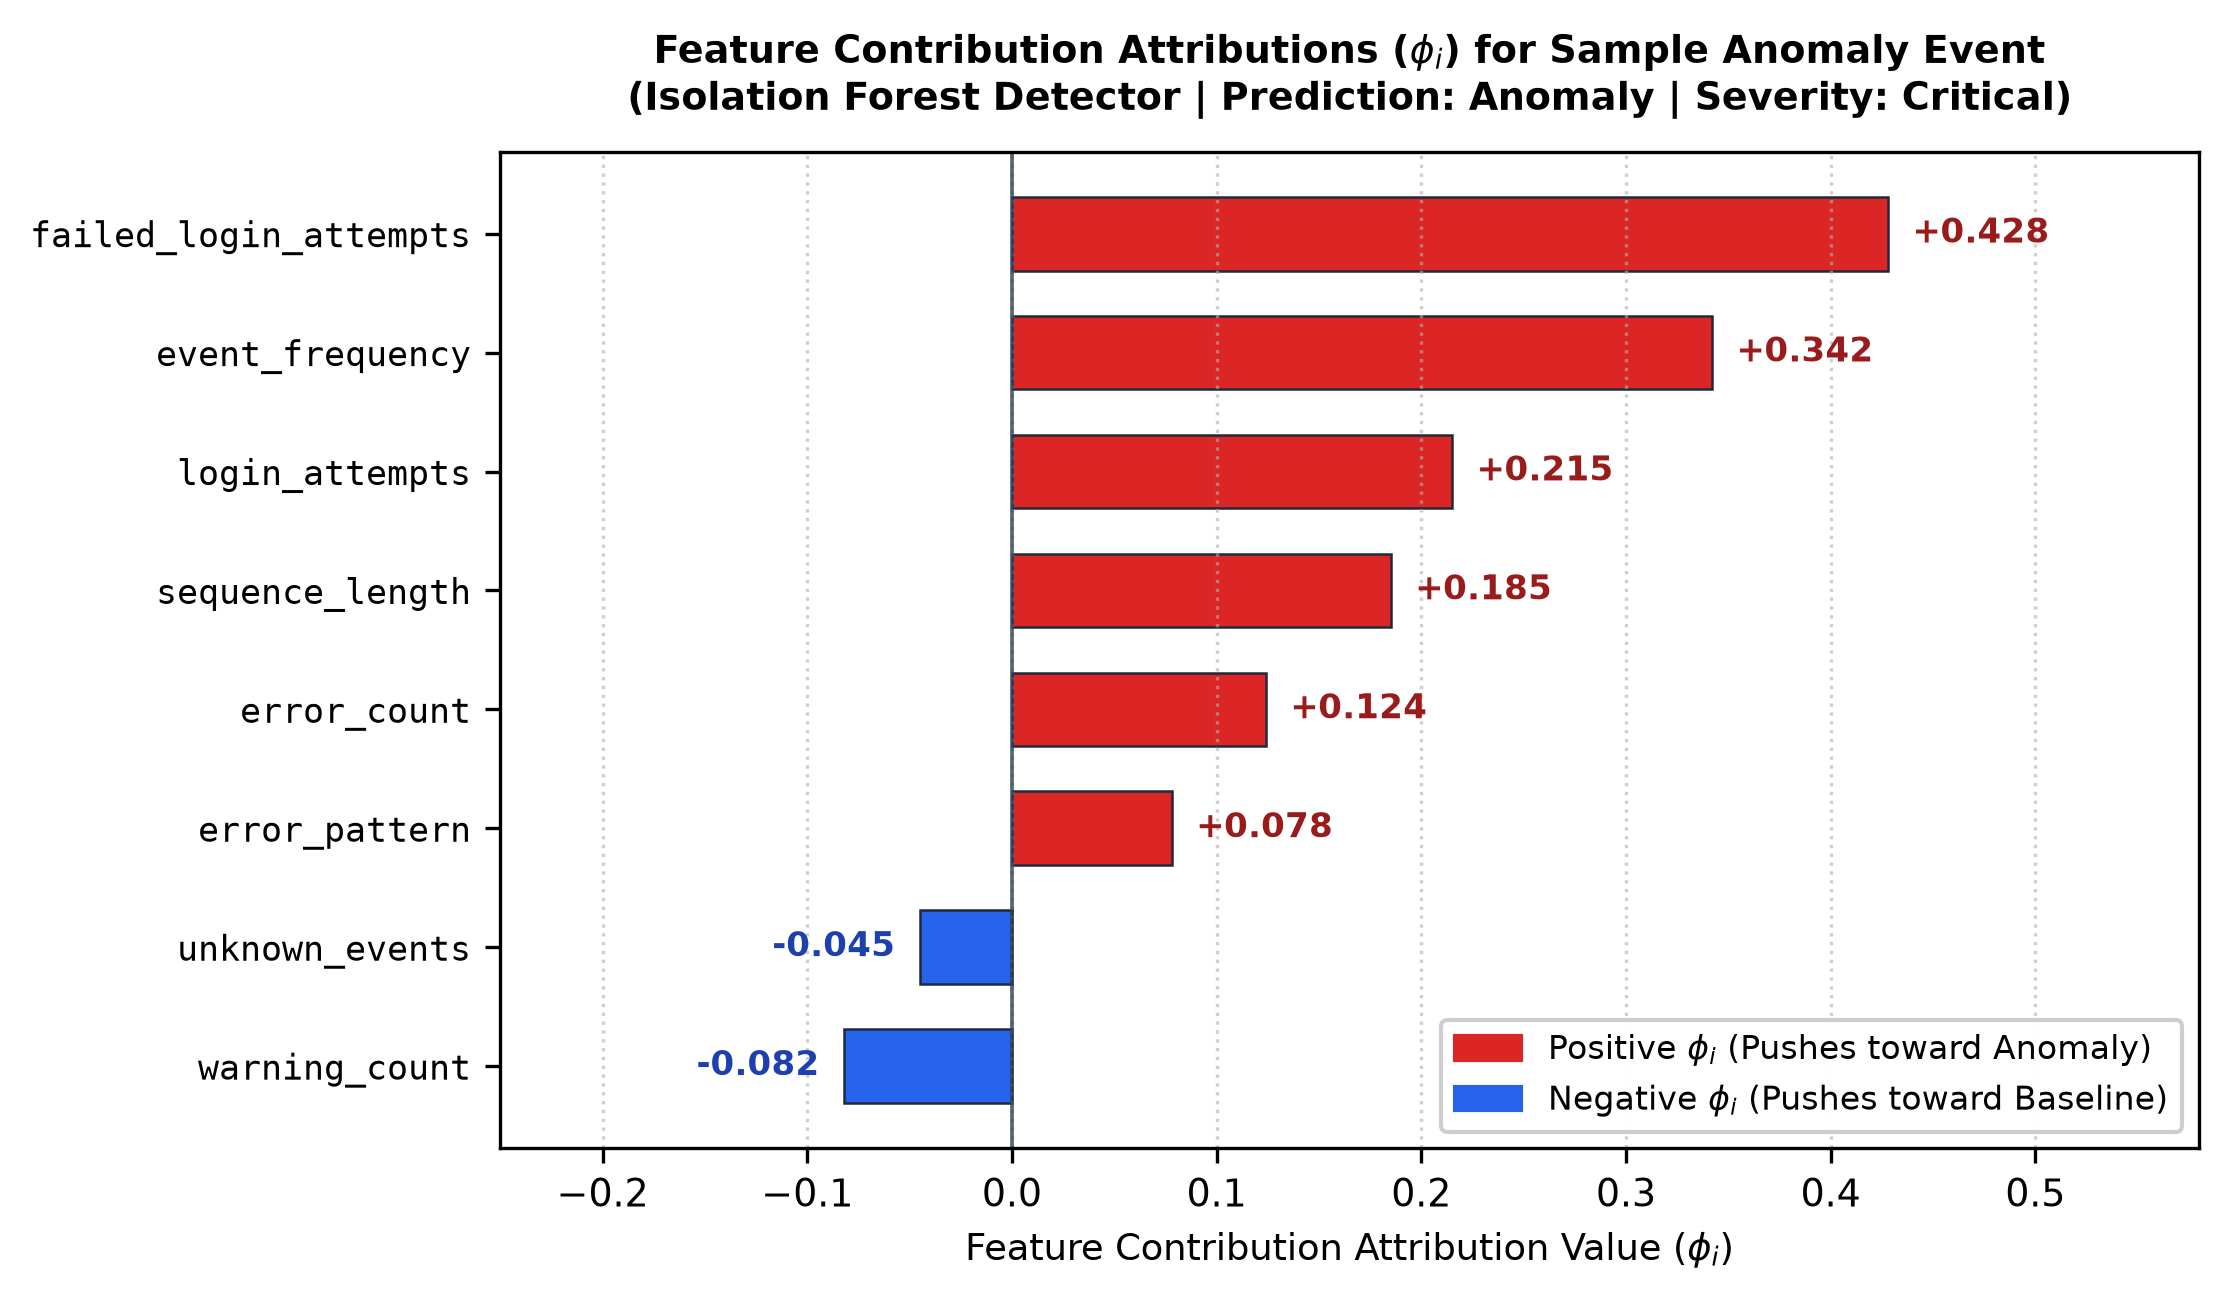
\includegraphics[width=\columnwidth]{fig_shap.png}
\caption{Feature contribution attributions ($\phi_i$) decomposing model anomaly scores across behavioral features to provide interpretability for detected anomalies.}
\label{fig_shap}
\end{figure}

\section{Limitations}
\label{sec:limitations}
While Smart-Log demonstrates effective unsupervised detection capabilities on the evaluated datasets, several limitations should be noted:
\begin{enumerate}
\item \textbf{Recall Reduction in Consensus Mode:} In the evaluated scenario experiment, the dual-model consensus state reduced recall to 14.67\%, meaning it functions as a complementary high-confidence triage filter rather than a standalone replacement for the primary anomaly detector.
\item \textbf{Static Windowing:} The sliding window size ($W=5$) is fixed; adaptive temporal windowing could improve sensitivity across varying log throughputs.
\item \textbf{Single-Host Context:} The current feature schema operates on host-level log streams and does not yet correlate multi-host distributed attack graphs across cloud networks.
\end{enumerate}

\section{Conclusion}
\label{sec:conclusion}
In this paper, we presented \textbf{Smart-Log}, an unsupervised and explainable log anomaly detection framework for server security. By projecting syslog events into an 8-dimensional behavioral feature space over sliding temporal windows, the framework captures operational dynamics without using anomaly labels as training targets. 

The evaluation indicates that Isolation Forest is the stronger primary detector among the evaluated models, achieving ROC-AUC values above 0.96 on both experimental datasets. The dual-model configuration provides an additional decision-consensus mechanism for high-confidence triage, while the explainability layer provides feature-level attribution for anomaly analysis. Future work will investigate streaming online adaptation and multi-host distributed log correlation for enterprise environments.

\section*{Acknowledgment}
The authors would like to thank the Department of Computer Science and Engineering at Bapuji Institute of Engineering and Technology, Davanagere, for providing computational resources and academic support for this project.

The authors acknowledge the use of artificial intelligence (AI) language tools during manuscript preparation. The tools were used to assist with language refinement, organization, LaTeX formatting, and technical writing support. The authors reviewed and verified all content, including the methodology, implementation details, experimental results, and references, and remain fully responsible for the accuracy and integrity of the manuscript.

\begin{thebibliography}{00}
\fontsize{9pt}{11pt}\selectfont
\setlength{\itemsep}{2pt plus 0.5pt minus 0.5pt}

\bibitem{b1} R. Dwivedi, N. Gupta, and A. Shrivastava, ``Anomaly identification in cyber logs through machine learning techniques,'' \emph{Int. Res. J. Eng. Appl. Sci. (IRJEAS)}, vol. 13, no. 4, 2025, doi: 10.55083/irjeas.2025.v13i04002.

\bibitem{b2} N.-A. Maspo, M. T. G. Hussain, A. S. Lone, and Z. S. M. A. Bashi, ``Anomaly detection of denial-of-service network traffic attacks using autoencoders and isolation forest,'' \emph{Int. J. Perceptive Cogn. Comput. (IJPCC)}, vol. 12, no. 1, pp. 145--151, 2026, doi: 10.31436/ijpcc.v12i1.680.

\bibitem{b3} A. Farzad and T. A. Gulliver, ``Unsupervised log message anomaly detection,'' \emph{ICT Express}, vol. 6, no. 3, pp. 229--237, 2020, doi: 10.1016/j.icte.2020.06.003.

\bibitem{b4} K. Sharma and V. Yelleti, ``Log anomaly detection via meta-learning and prototypical networks for cross domain generalization,'' \emph{arXiv preprint arXiv:2601.14336}, 2026.

\bibitem{b5} D. Patel, ``LLM-enhanced log anomaly detection: A comprehensive benchmark of large language models for automated system diagnostics,'' \emph{arXiv preprint arXiv:2604.12218}, 2026.

\bibitem{b6} H. Huang, P. Wang, J. Pei, J. Wang, S. Alexanian, and D. Niyato, ``Deep learning advancements in anomaly detection: A comprehensive survey,'' \emph{arXiv preprint arXiv:2503.13195}, 2025.

\bibitem{b7} N. A. Nipa, N. Bouguila, and Z. Patterson, ``A comparative study of log-based anomaly detection methods in real-world system logs,'' in \emph{Proc. 10th Int. Conf. Internet Things, Big Data Security (IoTBDS)}, 2025, pp. 141--152, doi: 10.5220/0013367000003944.

\bibitem{b8} W. Li, Y. Wu, W. Huang, F. Zhou, W. Ou, H. Wang, and L. Deng, ``System log anomaly detection based on contrastive learning and retrieval-augmented,'' \emph{Sci. Rep.}, vol. 15, 2025, doi: 10.1038/s41598-025-22208-7.

\bibitem{b9} M. Bekkouche and S. M. Benslimane, ``Improving anomaly detection in the HDFS dataset,'' [Online]. Available: \url{https://mdbekkouche.github.io/}

\bibitem{b10} M. Bekkouche and S. M. Benslimane, ``Improving anomaly detection in the HDFS dataset with novel machine learning models and techniques,'' \emph{Comput. Sci. J. Moldova}, vol. 33, no. 3, pp. 322--351, 2025, doi: 10.56415/csjm.v33.16.

\bibitem{b11} C. Wang, Z. Li, M. Ma, and P. Chen, ``Log2Graphs: An unsupervised framework for log anomaly detection with efficient feature extraction,'' \emph{arXiv preprint arXiv:2307.00527}, 2023.

\bibitem{b12} S. Wang, R. Jiang, Z. Wang, and Y. Zhou, ``Deep learning-based anomaly detection and log analysis for computer networks,'' \emph{arXiv preprint arXiv:2407.05639}, 2024.

\bibitem{b13} L. Zhang, T. Jia, K. Wang, M. Jia, Y. Yong, and Y. Li, ``Reducing events to augment log-based anomaly detection models: An empirical study,'' in \emph{Proc. ACM/IEEE Int. Symp. Empir. Softw. Eng. Meas. (ESEM)}, 2024, pp. 538--548, doi: 10.1145/3674805.3695403.

\bibitem{b14} F. Leveni, G. W. Cassales, B. Pfahringer, A. Bifet, and G. Boracchi, ``Online isolation forest,'' in \emph{Proc. 41st Int. Conf. Mach. Learn. (ICML)}, PMLR vol. 235, 2024, pp. 27288--27298.

\bibitem{b15} Z. Chen, J. Liu, W. Gu, Y. Su, and M. R. Lyu, ``Experience report: Deep learning-based system log analysis for anomaly detection,'' \emph{arXiv preprint arXiv:2107.05908}, 2021.

\bibitem{b16} M. Landauer, S. Onder, F. Skopik, and M. Wurzenberger, ``Deep learning for anomaly detection in log data: A survey,'' \emph{Mach. Learn. Appl.}, vol. 12, Art. no. 100470, 2023, doi: 10.1016/j.mlwa.2023.100470.

\bibitem{b17} M. Du, F. Li, G. Zheng, and V. Srikumar, ``DeepLog: Anomaly detection and diagnosis from system logs through deep learning,'' in \emph{Proc. ACM SIGSAC Conf. Comput. Commun. Secur. (CCS)}, 2017, pp. 1285--1298, doi: 10.1145/3133956.3134015.

\bibitem{b18} Q. Huang, J.-G. Lou, Y. Wang, Q. Lin, and D. Zhang, ``LogAnomaly: Unsupervised detection of sequential and quantitative anomalies in unstructured logs,'' in \emph{Proc. 28th Int. Joint Conf. Artif. Intell. (IJCAI)}, 2019, pp. 4739--4745.

\bibitem{b19} H. Guo, S. Yuan, and X. Wu, ``LogBERT: Log anomaly detection via BERT,'' in \emph{Proc. Int. Joint Conf. Neural Netw. (IJCNN)}, 2021, pp. 1--8, doi: 10.1109/IJCNN52387.2021.9534113.

\bibitem{b20} A. Javaid, Q. Niyaz, W. Sun, and M. Alam, ``A deep learning approach for network intrusion detection system,'' in \emph{Proc. EAI}, 2016, doi: 10.4108/eai.3-12-2015.2262516.

\bibitem{b21} T. Nguyen and M. Aiello, ``Anomaly detection in cybersecurity logs using deep autoencoders,'' \emph{Future Gener. Comput. Syst.}, vol. 112, pp. 580--595, 2020, doi: 10.1016/j.future.2020.09.018.

\bibitem{b22} A. Sharma and S. Mukhopadhyay, ``Anomaly detection using isolation forest and K-means clustering,'' in \emph{Proc. IEEE Int. Conf. Comput. Commun. E-Technol. (ICCCET)}, 2020, doi: 10.1109/ICCES48766.2020.9225482.

\bibitem{b23} P. Goyal, A. Bansal, and D. Tomar, ``Anomaly detection for cyber security using LSTM and GRU,'' in \emph{Proc. IEEE 4th Int. Conf. Adv. Comput. Commun. Control Netw. (ICAC3N)}, 2022, pp. 885--889, doi: 10.1109/ICAC3N56670.2022.10192808.

\bibitem{b24} H. Miao, J. Ding, and L. Zhang, ``A hybrid model for log anomaly detection based on CNN and attention mechanism,'' in \emph{Proc. IEEE Int. Conf. Big Data}, 2022, pp. 2481--2488, doi: 10.1109/BigData55660.2022.10004843.

\end{thebibliography}

\end{document}
